\section{Models and Algorithms}\label{tes}
In this section various Voronoi algorithms, namely the incremental, divide and conquer, and Fortune's algorithm are considered, as well as clustering methods for grouping points in a space. Concepts and notation used in the explanation of these algorithms are also discussed
%--------------------------------------------------------------------------------------
\subsection{Voronoi Tessellations}\label{tes:sec:vor}
A Voronoi tessellation is a partitioning of a space $S$ by a set of points. Given $n$ points (seed points) the space, $P = \{p_0,p_2,...,p_{n-1}\}, P \subset S$, is partitioned into $n$ regions, known as Voronoi regions or Voronoi cells, where every point, $s \in S_i,0 \leq i \leq n-1$ in a region, $S_i \subset S$, is closest to a single seed point, $p_i \in P$, in terms of the space's distance measurement operation, $d$ \citep{okabe2009spatial}. An example of a Voronoi diagram is illustrated in Figure \ref{tes:fig:voreg}.
%
\begin{figure}[H]
    \centering
    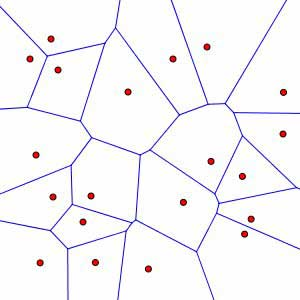
\includegraphics[scale=0.65]{Images/voronoi.jpg}
    \caption[]{Voronoi diagram\footnotemark}
    \label{tes:fig:voreg}
\end{figure}
\footnotetext{Taken from \url{http://www.ams.org/samplings/feature-column/fcarc-voronoi}}
%
\subsubsection{Weighted Voronoi Tessellations}\label{tes:ssec:wei}
The basic form of the Voronoi tessellation has the seed points being indistinguishable from one another, other than having a different position in the space. An extension of the tessellation is with the seeds having some bias or weighting associated with them. These weightings can represent a property of the data, for example, in terms of radio interferometry, they can represent the intensity of each detected source. This weighting can affect $d$ in different ways, depending on how the weighting is accounted for; this is know as the ``weighted distance''. Some of the methods, discussed in \citet{okabe2009spatial} include multiplicative, additive, compound and power Voronoi diagrams. These diagrams have distance operators described below as $d_M$, $d_A$, $d_C$, and $d_P$, respectively.
%
\begin{equation*}
\begin{aligned}
  d_M(s,p_i) &= \frac{1}{w_i}d			\\
  d_A(s,p_i) &= d - w_i				\\
  d_C(s,p_i) &= \frac{1}{w_{i1}}d - w_{i2}	\\
  d_P(s,p_i) &= d^2 - w_i			\\
\end{aligned}
\end{equation*}
%
Problems arise in attempting to compute the tessellations for the multiplicative, additive and compound Voronoi diagrams as the edges of these diagrams could potentially be curved by a circular arc ($d_M$,$d_C$), a hyperbolic arc ($d_A$,$d_C$) or a fourth order polynomial arc ($d_C$) \citep{okabe2009spatial}. This leaves the power diagram as the only Voronoi diagram that enforces straight lines for the edges and the resulting tessellation as a set of convex polygons, similar to the standard Euclidean Voronoi diagram. For the power diagram, if the weighting is equal for all points, the resulting diagram is the same as that of a standard Euclidean Voronoi diagram. It is however possible in the power diagram, that a seed point will not be contained within its own associated Voronoi polygon. This occurs when two seed points ($p_i,p_j \in P$, $w_i<w_j$, $i\neq j$) are close enough together such that the weighted bisector, defined by 
%
\begin{equation}
 b(p_i,p_j) = \frac{1}{2}(||\vec{x}_i||^2-||\vec{x}_j||^2+w_i-w_j) \qquad \vec{x}_i = (x_i,y_i),
\end{equation}
%
does not lie on the line segment $\bar{p_ip_j}$. When this occurs, $p_i$ lies in the region of $V_j$. If the difference in weighting between $p_i$ and $p_j$ is large enough and the distance between them small enough, the points in $V_i$ may be an empty set. It is worth noting that Power Diagrams are also referred to as General Voronoi Diagrams \citep{aurenhammer1987power}.
%--------------------------------------------------------------------------------------
\subsection{Voronoi Tessellation Generation Algorithms}\label{tes:sec:tga}
Although Voronoi tessellations extend to multiple dimensions, for simplicity we only discuss those in a two dimensional plane.
%
\subsubsection{Incremental Algorithm}\label{tes:ssec:inc}
The most simplistic of the generation algorithms, the Incremental is an iterative algorithm as described below \citep{green1978computing} \citep{okabe2009spatial}:
\begin{enumerate}
\item Start from $i=0$ with an empty plane.
\item\label{tes:itm:inc:add} A seed point, $p_i$ is placed into the plane.
\item The nearest neighbouring seed point $p_f=p_{nn}$ is found.
\item\label{tes:itm:inc:bis} A perpendicular bisector is drawn between $p_i$ and $p_f$ (if it exists).
\item The bisecting line is followed in both directions until it intercepts an existing edge or the plane's boundary on both ends.
\item A new edge is defined by this segment of the bisector as part of both $p_i$ and $p_f$.
\item The seed point of the polygon that shares the found edge clockwise to $p_f$ (anticlockwise to $p_i$) is set to $p_f$.
\item Continue from step \ref{tes:itm:inc:bis} until $p_f=p_{nn}$.
\item Set $i = i +1$ and repeat from step \ref{tes:itm:inc:add} until $i=n$.
\end{enumerate}
In its most naive form, this algorithm achieves an efficiency of $O(n^2)$.
%
\subsubsection{Divide and Conquer Algorithm}\label{tes:ssec:dac}
The Divide and Conquer algorithm was first proposed by \citet{shamos1975closest}, but is also described in \citep{okabe2009spatial}. It is a recursive algorithm that improves on the Incremental algorithm by having an execution time of $O(n\log n)$.
\begin{enumerate}
\item If the space contains only one point, return it with the entire plane as its Voronoi region.
\item Divide the space, $S$ containing the set of $n$ seed points, $P$, into two subspaces, $S_L$ and $S_R$, such that $S_L$ and $S_R$ contain $n/2$ seed points and every seed point of $P_L$ lies to the left of every seed point of $P_R$ (this is made easier if $P$ is ordered).
\item Recursively compute the Voronoi tessellations for $P_L$ in $S_L$ and $P_R$ in $S_R$; called $V_L$ and $V_R$, respectively.
\item A polygonal line, $Q$, must now be found such that $Q$ merges $V_L$ and $V_R$ into a single Voronoi tessellation, $V$:
\begin{enumerate}
 \item Start with the polygon of $V_R$ which contains the top-left corner of $S_R$, $p_R$ and the polygon of $V_L$ which contains the top-right corner of $S_L$, $p_L$. Since $p_L$ must lie to the left of $p_R$, they must overlap when $V_L$ and $V_R$ are extended into $S$.
 \item\label{tes:itm:dac:bis} A perpendicular bisector is drawn between $p_L$ and $p_R$ and segmented between its two closest edge intercepts from the shortest distance between $p_L$ and $p_R$. This segment is added to $Q$.
 \item If the lower edge, intercepted by the bisector is in $V_R$, $p_R$ is set to the seed point polygon which shares this edge and similarly if the edge is in $V_L$.
 \item Continue from step \ref{tes:itm:dac:bis} until the bottom of $S$ is reached.
\end{enumerate}
\item Remove all line segments of $V_L$ to the right of $Q$ and all those of $V_R$ to the left of $Q$ to form $V$.
\item Return $V$ recursively until the full Voronoi tessellation is complete.
\end{enumerate}
Part of achieving this efficiency is assuming $P$ is co-lexicographically ordered, meaning for all $p_i,p_j \in P$, $0 \leq i < j < n$; $x_i > x_j$ or $(x_i = x_j$ and $y_i > y_j)$. This speeds up the partitioning of $P$ into $P_R$ and $P_L$ at each level of recursion.
%
\subsubsection{Fortune's Algorithm (Sweep-Line Method)}\label{tes:ssec:fort}
\citet{fortune1987sweepline} describes an algorithm where the tessellations are found by a line ``sweeping'' over the space and solving the problem at each step of the sweep. This can be problematic for Voronoi tessellations as the line may intercept the Voronoi region of a seed point before it intercepts the point. Therefore the Voronoi tessellation is not computed directly, but through a geometric transform. The transform $\phi(x(s),y(s))$ works such that for any point, $s \in S$ with coordinates $(x(s),y(s))$, 
\begin{equation}
  \phi(x(s),y(s)) = (x(s) + r(s), y(s)),
\end{equation}
where $r_i(s)$ is defined as the distance to the seed point $p_i \in P$ and $r(s) = min\{r_i(s) | 1 \leq i \leq n-1\}$, is the distance to the closest seed point to $s$. This transform can easily be reversed to re-obtain $S$ and its set of Voronoi tessellations. Now, for the transform of $S$, $\phi(S)$ denoted by $\Phi$, the left-most point of each Voronoi Region is its seed point (except the left-most seed point); this is essential for the algorithm. It is important to note that the perpendicular bisectors of seed points in $S$, through the transform, become hyperbolas in $\Phi$ (provided they are not horizontal in $S$). For $p_i,p_j\in P$, the hyperbola is denoted as $h_{ij}$ which can be split into $h^+_{ij}$ and $h^-_{ij}$ as the upper and lower half-hyperbolas about the left-most point, respectively. Set $Q$ is denoted as the set of all event points in the algorithm. $Q$ is initially populated with the seed points (in co-lexicographical order) but the edge interceptions are added as they are found. The algorithm, as described by \citet{okabe2009spatial} is as follows:
\begin{enumerate}
  \item Add $P$ to $Q$.
  \item Choose and delete the leftmost seed point, $p_i$ from $Q$.
  \item Create a list, $L$ containing the transformed Voronoi region of $p_i$, $\phi(V_i)$.
  \item\label{tes:itm:for:q} While $Q$ is not empty do the following:
  \begin{enumerate}
    \item Choose and delete the leftmost element, $w$ of $Q$.
    \item If $w$ is a seed point:
    \begin{enumerate}
      \item Set $p_i=w$.
      \item Find the region, $\phi(V_j)$, containing $p_i$.
      \item Replace $\phi(V_j)$ in $L$ with $(\phi(V_j),h^-_{ij},\phi(V_i),h^+_{ij},\phi(V_j))$.
      \item Find the half-hyperbola intercept(s) with any other hyperbolas, if they exist, and append these to the front of $Q$.
      \item Repeat from step \ref{tes:itm:for:q}.
    \end{enumerate}
    \item If $w$ is a half-edge:
    \begin{enumerate}
      \item Set $\phi(q_t)=w$ where $\phi(q_t)$ is the intercept of $h^\pm_{ij}$ and $h^\pm_{jk}$.
      \item Replace all sequences of the form ($h^\pm_{ij},\phi{V_j},h^\pm_{jk}$) on $L$ with $h=h^+_{ik}$ or $h=h^-_{ik}$ appropriately.
      \item Remove from $Q$ any intersections of $h^\pm_{ij}$ and $h^\pm_{jk}$ with other half-hyperbolas.
      \item Move any intersections of $h$ in $L$ to $Q$.
      \item\label{tes:itm:for:mark} Mark $\phi(q_t)$ as a Voronoi vertex incident to $h^\pm_{ij}$, $h^\pm_{jk}$ and $h$.
      \item Repeat from step \ref{tes:itm:for:q}.
    \end{enumerate}
  \end{enumerate}
  \item Return the half-hyperbolas on $L$, the set of marked intersections from step \ref{tes:itm:for:mark} and the relations among them.
\end{enumerate}
%--------------------------------------------------------------------------------------
\subsection{Clustering Algorithms} \label{tes:sec:clu}
It may be the case that the number of potential seed points in a space, $N_p$, is much larger than the optimal number of facets, $N_v$. In these cases the overall computation time would be drastically reduced if the $N_p$ points were grouped into $N_v$ clusters. From each of these clusters, a point is chosen as a seed point to be used to find the corresponding Voronoi tessellation. Some key examples of such clustering algorithms are described in this subsection.
%
\subsubsection{K-Means Algorithm}\label{tes:ssec:kma}
K-means clustering is an iterative process where an initial guess at the center of a cluster, $c$, is made and improved with each iteration. It is named as such because it seeks to separate $n$ objects into $k$ clusters where, for each object in a cluster $( o^i \in C_i$, $i \in \mathbb{R}$, $0\leq i \leq k-1)$ the mean point of that cluster, $c_i$, is closer to it than any other mean point and the $c_i$ is representative of the average values of all points, $\frac{1}{m}\sum^m_{j=1}o^i_j$, in $C_i$. \citet{way2012advances} describe the algorithm as follows:
\begin{enumerate}
  \item	Randomly choose $k$ mean points $(c_0,\dots,c_{k-1})$.
  \item\label{tes:itm:km} Assign each $c_i$ an empty object set, $C_i$.
  \item Iterate through all the objects in the space $(o_0,\dots,o_{n-1})$ and assign the object to the object set of the mean point closest to it.
  \item Set all $c_i$ to be the average of all points in their respective $C_i$.
  \item If the sum of the changes in $c_i$, $\sum_0^{k-1} \Delta c_i$, is greater than some given tolerance, $\epsilon$, the algorithm is repeated from step \ref{tes:itm:km}, else return the set of means (and their object sets if 	      necessary).
\end{enumerate}
One obvious problem with this algorithm is that the number of iterations can be unpredictable; this is addressed by having the sum of changes only converge to $\epsilon$, instead of complete convergence. With large data sets and large $k$-values where the mean points converge in smaller steps with every iteration, this can drastically reduce the runtime of the algorithm. The clusters produced are also dependent on the initial placement of the mean points \citep{way2012advances}. Other methods of improving the runtime include probabilistic choices of starting mean points \citep{arthur2007k} and constraining the distance and using the triangle inequality \citep{hamerly2010making}.
%
\subsubsection{Bisecting K-Means Algorithm}\label{tes:ssec:bkma}
A variation on the k-means algorithm is to embed it into another iterative method, which, by design, reduces the computation time and also improves the quality of the clusters produced. The algorithm works by branching large clusters into smaller ones. The algorithm, described by \citet{steinbach2000comparison}, is as follows:
\begin{enumerate}
  \item Start with the entire set of objects in the space as part of a single cluster.
  \item\label{tes:itm:bkm} Choose the largest cluster in the space.
  \item Split the objects into two sub-clusters and refine iteratively by way of the k-means algorithm.
  \item Repeat from step \ref{tes:itm:bkm} until $k$ clusters are produced.
\end{enumerate}
%
\subsubsection{Agglomerative Clustering Algorithm}
Differing from the k-means algorithm (and more specifically the bisecting k-means) is the agglomerative clustering algorithm. Instead of starting with a single cluster containing all points, this algorithm instead places every point in its own cluster and merges them until the required number of clusters are produced. \citet{way2012advances} describe the algorithm as:
\begin{enumerate}
  \item Begin with each object in its own cluster.
  \item\label{tes:itm:aca} Merge the two closest clusters.
  \item Repeat step \ref{tes:itm:aca} until $k$ clusters remain.
\end{enumerate}
Although this algorithm will always yield the same result for a given data set, it is far more expensive than the k-means. Improvements can be made on this, however by instead building a minimum spanning tree, weighted by the distance between the data and iteratively removing the links with the highest weights until the number of required clusters is produced.
%--------------------------------------------------------------------------------------
\subsection{Related Work}\label{ra:sec:rw}
%
\subsubsection{Standard Voronoi Faceting}\label{ra:ssec:svf}
In \citep{tasse2014applying}, \citep{smirnov2015radio} and \citep{van2016lofar}, a series of observed or simulated extragalactic points are clustered into facets using a Voronoi tessellation algorithm with the seed points for these facets set as the brightest points in each facet. An example of this can be seen in Figure \ref{tes:fig:stelvor} where the facets are superimposed over the source image from which they are derived.
%
\begin{figure}[H]
    \centering
    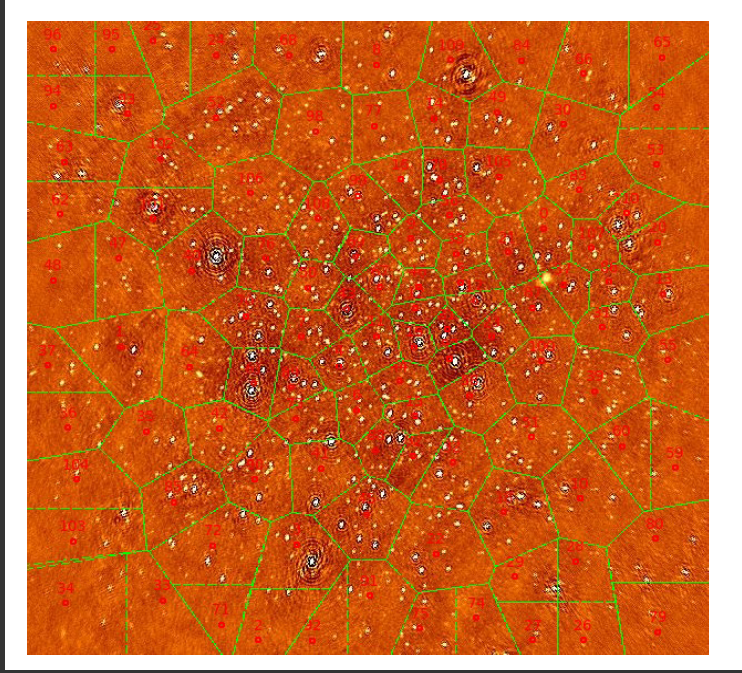
\includegraphics[scale=0.4]{Images/tessellation.png}
    \caption{Example of Voronoi faceting to group extragalactic points for Direction Dependant calibration.}
    \label{tes:fig:stelvor}
\end{figure}
%--------------------------------------------------------------------------------------